\subsection{实现指令流水线的硬布线控制器}
\subsubsection{实现原理}
\par
计算机的流水处理过程非常类似于工厂中的流水装配线,为了实现流水,首先把输入的任务分割为一系列子任务,并使各子任务能在流水线的各阶段并发的执行。当任务连续不断地输入流水线时,在流水线的输入端便连续不断地吐出执行结果,从而实现了子任务的并行性。
\par
用于该次实验的指令集中多为二节拍数指令,分别用于取值和执行,由于\tec 取指用总线和数据交换用总线并不会冲突,因此二节拍指令可将取值和执行并行执行,实现两级流水。三节拍指令仅有LD\comma ST两个指令,在第二三节拍均会使用到数据交换用总线,而\tec 仅具有一条数据交换用总线,为了防止总线占用冲突,可以和这两条指令并行执行的指令只有JC\comma JZ\comma STP三条,若仅对这三条指令采用三级流水效率提升并不高。
\subsubsection{实现方法}
\par 
经过小组组员的共同讨论,我们决定仅将指令周期分为两部分,分别为取指令和执行。
\par
对于一个包含n条指令的程序,若指令全为需要两个节拍数的指令,使用流水线需要n+1个节拍,而使用非流水线需要2n个节拍,当n趋于无穷时,加速比S趋于2;若指令全为需要三个节拍数的指令,使用流水线需要2n+1个节拍数,不使用流水线需要3n个节拍数,当n趋于无穷时,加速比S趋于1.5。
\par 
由于取值操作都已经放入指令周期的最后一个节拍电位与指令执行并行实现,因此我们在原有的指令集基础上添加了NOP指令,用于第一次进入程序时的取指,后续指令的取值放在前一条指令的最后一个节拍内,实现取指和执行的时间上并行。指令流程图如下:
\begin{figure}[hbt!]
    \centering
    \label{流水线指令流程图1}
    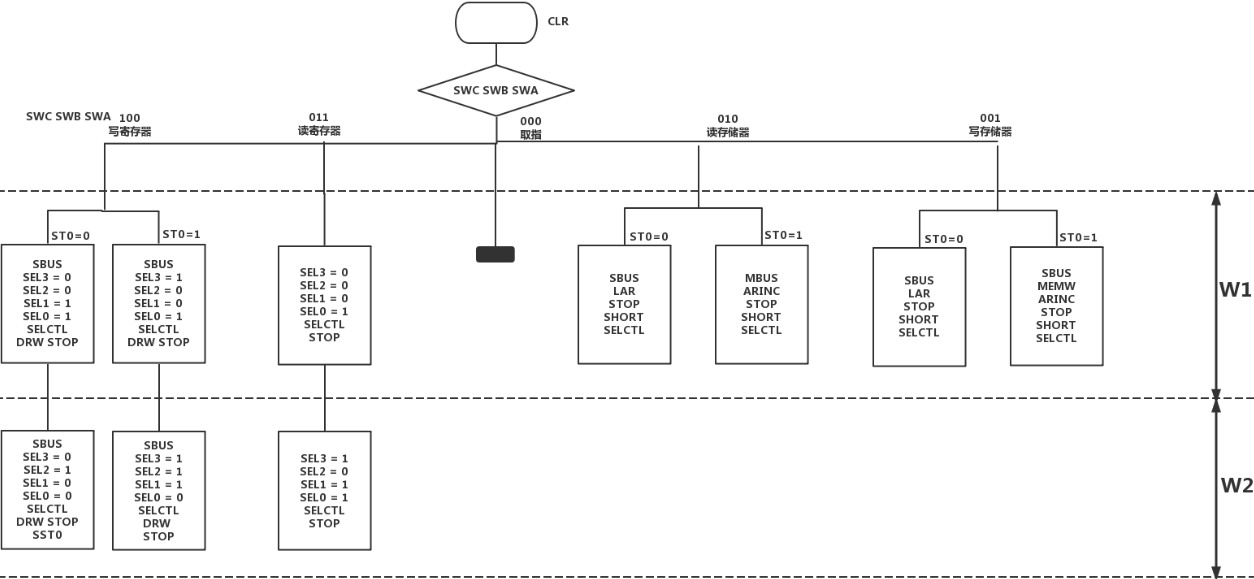
\includegraphics[width=\textwidth]{figures/chapter3/流水线指令流程图1.png}
\end{figure}
\newpage
\begin{figure}[hbt!]
    \centering
    \label{流水线指令流程图2}
    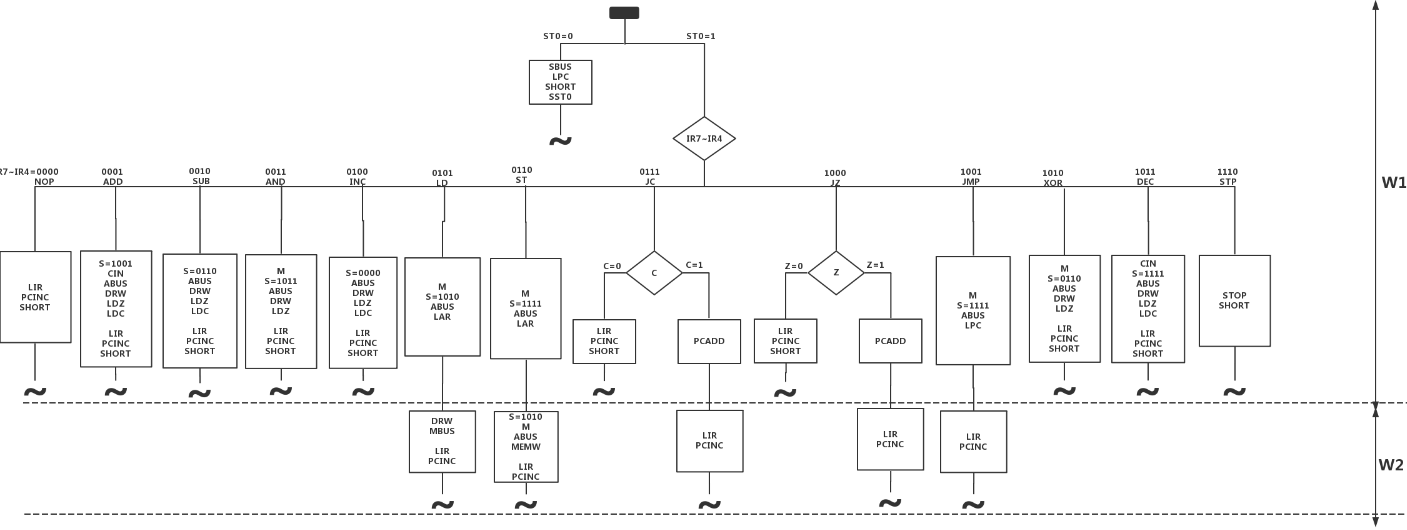
\includegraphics[width=\textwidth]{figures/chapter3/流水线指令流程图2.png}
    \caption{流水线指令流程图}
\end{figure}
\par
我们依据指令流程图修改了译码表,用于程序组合逻辑的实现,译码表修改部分如下:
\begin{figure}[hbt!]
    \centering
    \label{流水线译码表修改部分}
    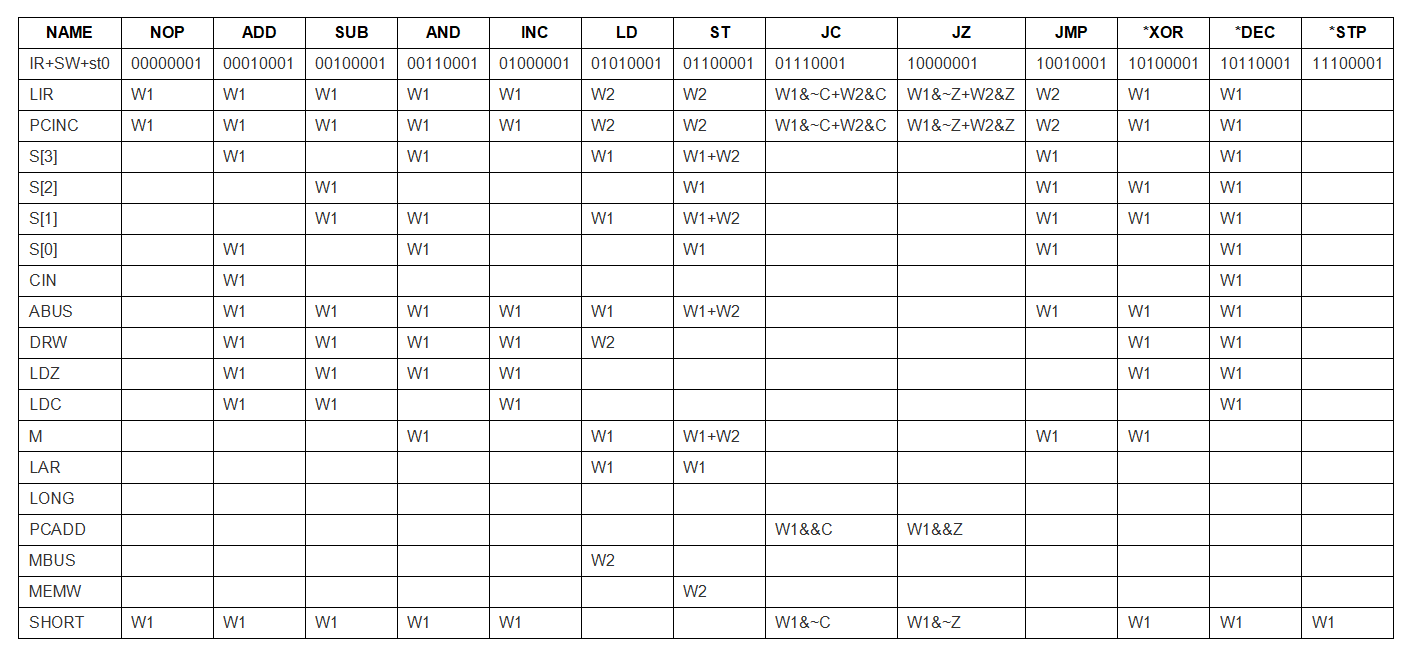
\includegraphics[width=\textwidth]{figures/chapter3/流水线译码表修改部分.png}
    \caption{流水线译码表修改部分}
\end{figure}


